\clearpage
\section{\textsc{Versuchsaufbau und Durchführung}}
\subsection{Vermessung der Signale am Oszilloskop}
Um die Signale mit dem Oszilloskop vermessen zu können, wurde es einmal direkt an den Photomultiplier (an den Preamplifier) angeschlossen und am Mainamplifier jeweils einmal am bipolaren und am unipolaren Ausgang.
\subsection{Aufnehmen der Energie-Spektren}
Hierzu wurde der unipolare Ausgang des MP mit dem Vielkanalanalysator (Multi Channel Analyser, MCA) verbunden, siehe Abbildung \ref{fig:spek_auf}. Die Spektren werden als Histogramm auf dem Computer aufgenommen, der MCA ordnet jedem Eingangsimpuls abhängig von dessen Pulshöhe einen Kanal zu. Um die Spektren interpretieren zu können werden die wird eine Energie-Eichung des MCAs durchgeführt, indem man Gauß-Kurven an die charakteristischen Peaks fittet und ermittelten Kanalnummern der Peaks gegen die Energie der Peaks aufträgt. Dieser Zusammenhang sollte linear sein.

\begin{figure}[h]
\begin{center}
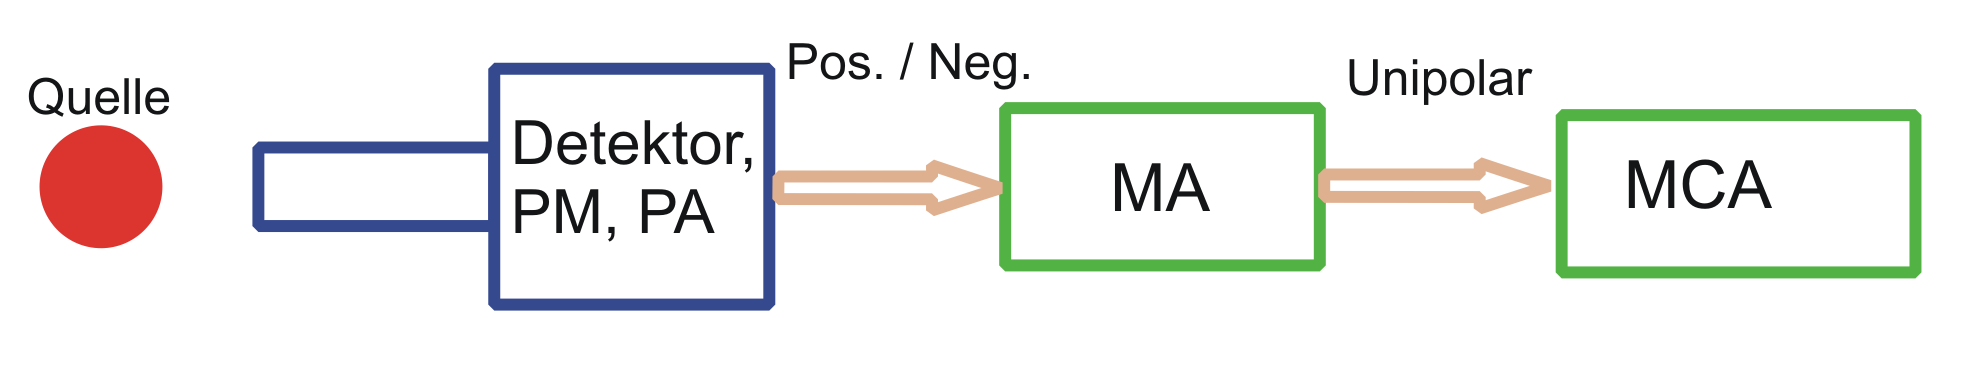
\includegraphics[scale=0.25]{energiespektren}
\caption{Schaltschema zum Aufnehmen der Energiespektren. Quelle: [ver]}
\label{fig:spek_auf}
\end{center}
\end{figure}
\subsection{Setzten der Energiefenster}
An einem Singel Channel Analyser (SCA) kann man ein Energiefenster angeben, dieser gibt dann nur Signale aus wenn ein Signal welches in diesem entsprechenden Energiefenster liegt bei ihm ankommt. Diese ist unabhängig von der Signalhöhe, man erhält somit nur die Information, dass ein Signal in diesem Fenster detektiert wurde. Nun wird das Energiefenster des einen SCA auf den Peak bei 14,4 keV (späteres Start-Signal) und das andere auf 122 keV (späteres Stopp-Signal) eingestellt werden für die Messung der verzögerten Koinzidenzen. Hier sollte beachtet werden, dass die Fenster nicht zu groß und nicht zu klein gewählt werden da sonst ungewollte Nebeneffekte dominierend auftreten. Der Aufbau wird wie in Abbildung \ref{fig:energiefenster} gesteckt.
\begin{figure}[h]
\begin{center}
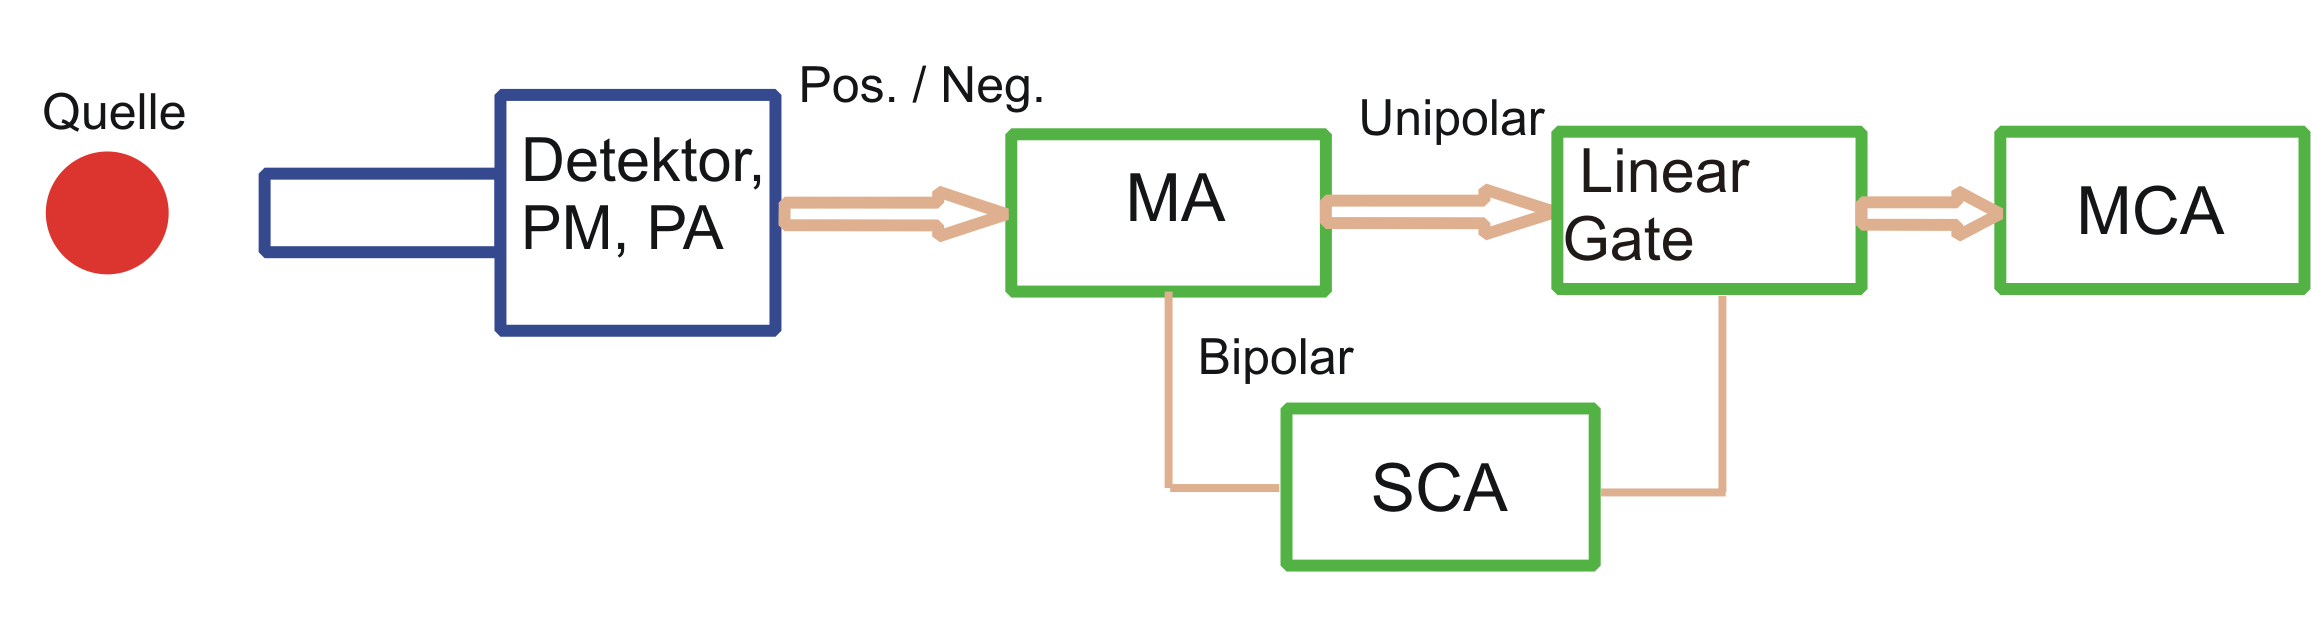
\includegraphics[scale=0.2]{energiefenster}
\caption{Schaltschema zum Einstellen der Energiefenster. Quelle: [ver]}
\label{fig:energiefenster}
\end{center}
\end{figure}
Bei diesem Aufbau leitet das Linear Gate die unipolaren Signal des MA nur an das MCA weiter, wenn ein Signal aus dem am SCA gewählten Energiefenster am SCA ankommt. Es muss darauf geachtet werden, dass das Delay am SCA auf den kleinsten Wert eingestellt wird damit die Signale von MA und SCA gleichzeitig beim Linear Gate ankommt und das MA Signal transmittiert wird.
\subsection{Messung der verzögerten Koinzidenzen}
Der Aufbau wird wie in Abbildung \ref*{fig:verzoegertauf} geschallten. Am TAC werden 5 $\mu s$ Eingestellt. Das 122keV-Signal soll durch die drei Delayboxen und die Verbindungskabel so verzögert werden, dass der Peak des Zeitspektrums etwa bei 4/5 des MCA-Kanalbereichs liegt. Falls nach mehreren Minuten noch keine Anzeichen von einem Peak zu erkennen so müssen die Einstellungen noch einmal geprüft werden. Ist jedoch ein Peak zu erkennen so soll die Messung mindestens 12 Stunden laufen. 
Aus dem Spektrum soll die Lebensdauer bzw. die Halbwertszeit des 14,4keV-Zustandes ermittelt werden. Beim linear aufgetragen Spektrum wird dies durch einen exponentiellen Fit und beim logarithmisch aufgetragen Spektrum durch einen Linearen Fit bestimmt. Jedoch soll vor dem Fitten der im nächsten Schritt gemessene Untergrund von den Messwerten abgezogen werden. 

\begin{figure}[h]
\begin{center}
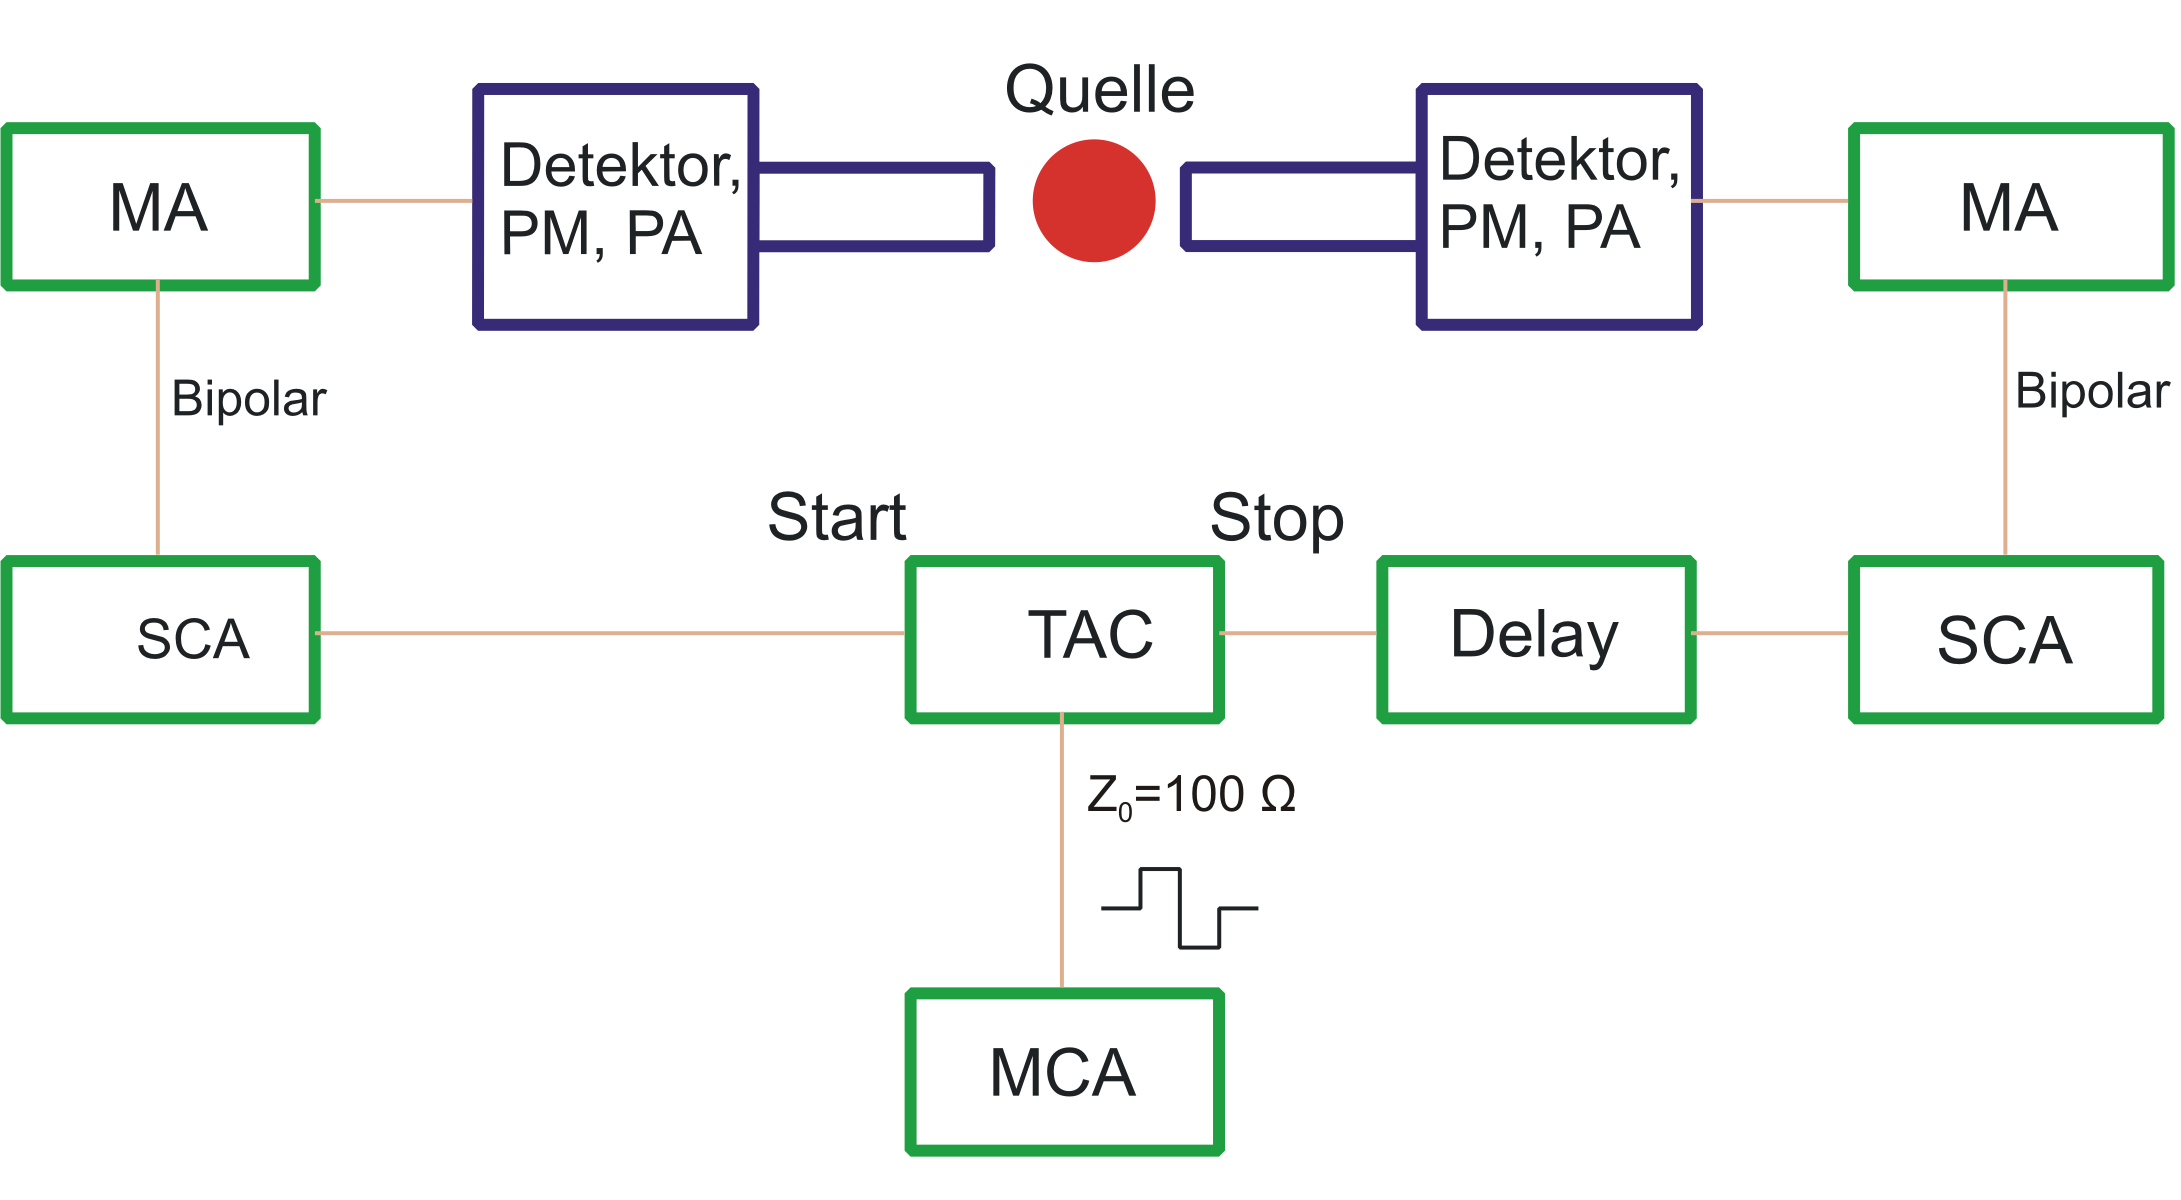
\includegraphics[scale=0.2]{verzoegertauf}
\caption{Schaltschema zum Messung der verzögerten Koinzidenzen. Quelle: [ver]}
\label{fig:verzoegertauf}
\end{center}
\end{figure}

\subsection{Messung der zufälligen Koinzidenzen}
Bei der Messung der zufälligen Koinzidenzen wird der selbe Aufbau wie bei den verzögerten Koinzidenzen benutzt, jedoch wird das Delay auf das 122keV Signal auf Null gesetzt und das vom 14,4keV auf einige hundert ns. Die Messung sollte einige Stunden dauern.
\subsection{Zeitkalibration des TAC}
Durch den Zeit-Impulshöhen-Konverter (Time to Amplitude Converter, TAC) erhält man durch ein Rechtecksignal die Zeitdifferenz zwischen Start- und Stoppsignal, welche durch die Höhe des Pulses ausgedrückt wird. Durch das erste Signal wird die Uhr gestartet, durch das Zweite wird die Uhr gestoppt. Da das MCA nur verschieden Energieniveaus erhält wird eine Zeitkalibration des TAC benötigt, damit den Kanälen die Zeitdifferenzen zugeordnet werden können.\\

Der Aufbau zur Zeitkalibration soll wie in Abbildung \ref{fig:aufbau_kal} erfolgen. Wie in der Skizze gezeigt wird das Ausgangssignal am SCA mit einem T-Stecker aufgeteilt. Dabei wir eines direkt an das Start-Eingang des TAC gelegt das andere wird über die Delayboxen an den Stopp-Eingang gelegt. Nun wird eine Messung zu verschiedenen Delayzeiten durchgeführt, wobei der Delay und die jeweils zum Delay ansprechenden Kanäle notiert werden (dies sind meistens nur ein oder zwei Kanäle), siehe Anhang, Abbildung \ref{fig:mess_kal}. Bei der Gegenüberstellung von Kanal zur entsprechenden Verzögerung sollte ein lineare Zusammenhang deutlich zu sehen sein. Dieser wird grafisch dargestellt.\\
\begin{figure}[h]
\begin{center}
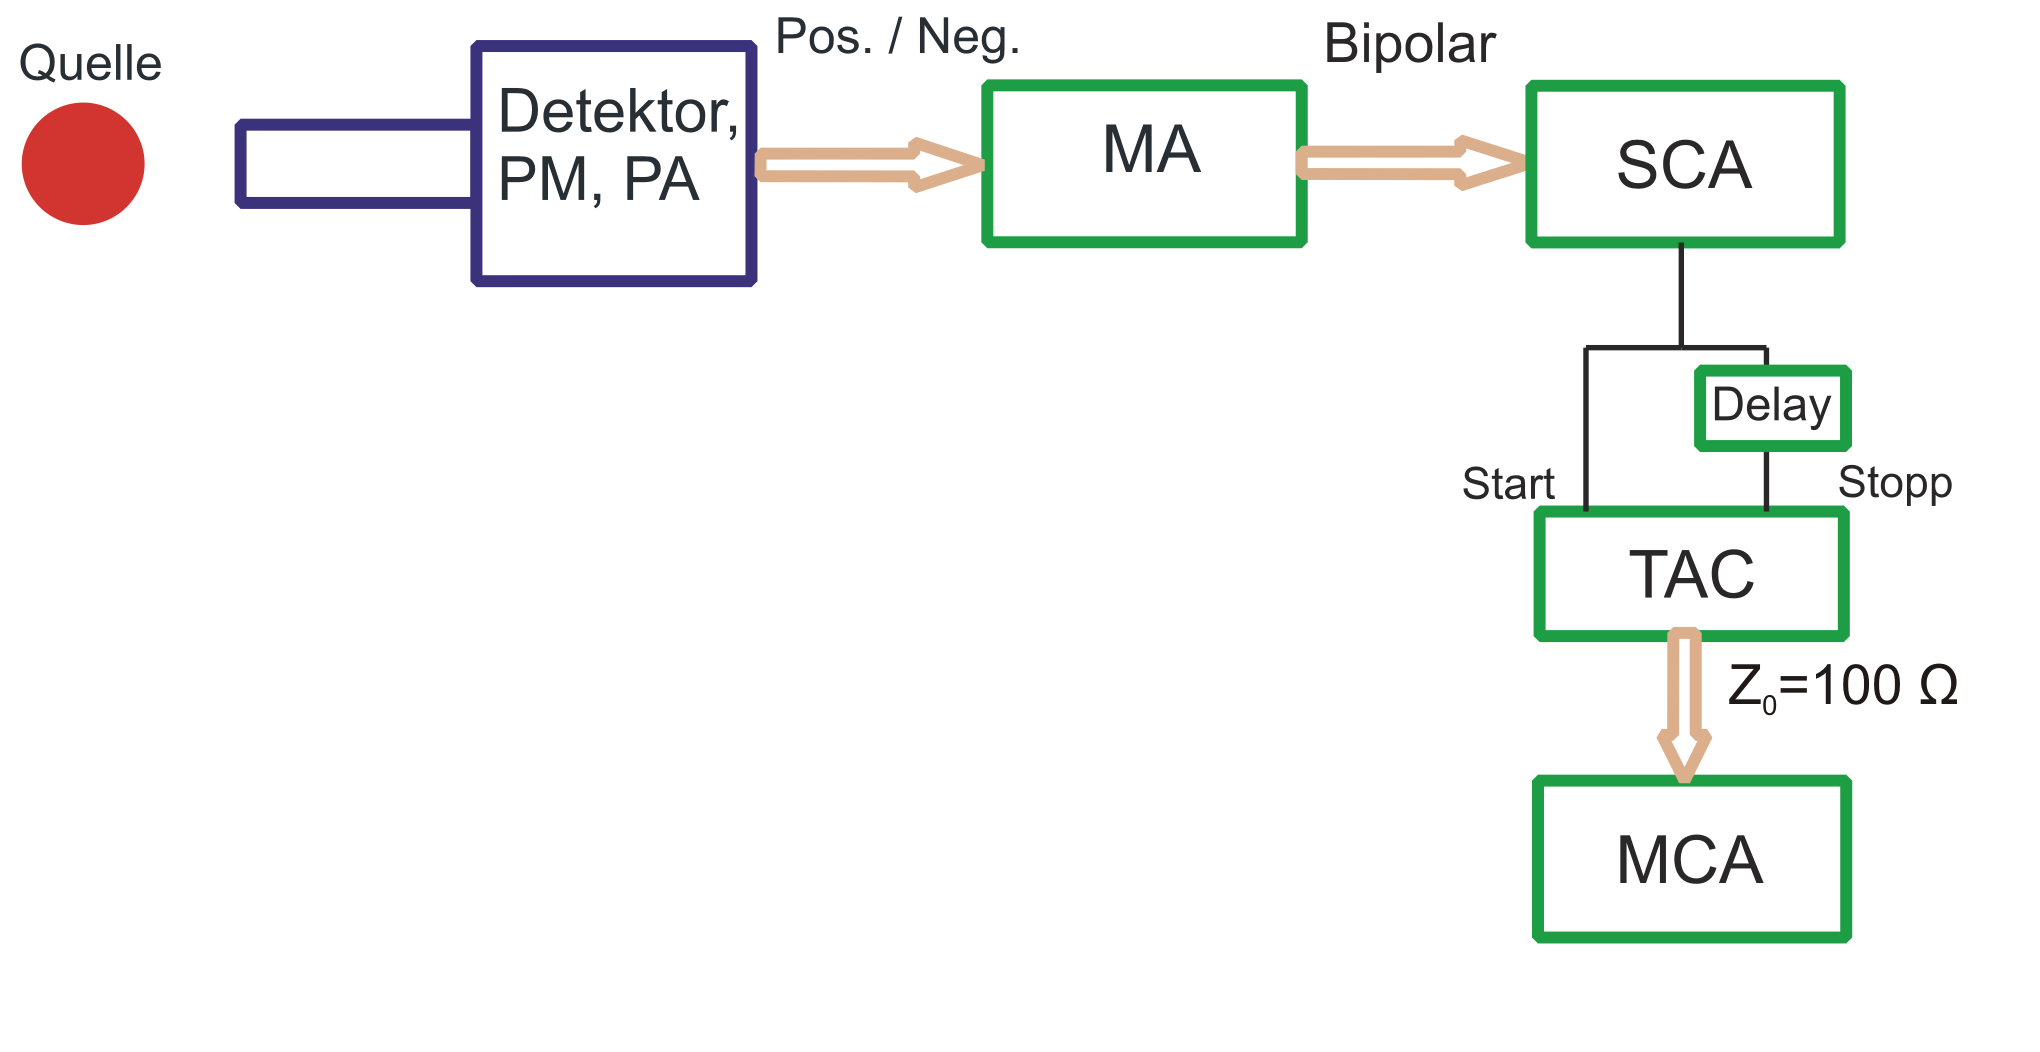
\includegraphics[scale=0.2]{aufbau_kal}
\caption{Funktionsweise des TAC. Quelle: [ver]}
\label{fig:aufbau_kal}
\end{center}
\end{figure}\\